\documentclass[11.5pt]{article}
\usepackage[utf8]{inputenc}
\usepackage[T1]{fontenc}
\usepackage[textwidth = 460pt,top = 80pt, bottom = 80pt]{geometry}
\usepackage{graphicx}
\usepackage[justification=default]{subfig} 
\usepackage[update]{epstopdf}
\usepackage[labelfont=bf]{caption}
\usepackage[dvipsnames]{xcolor}
\usepackage{fancyhdr}
\usepackage{booktabs}
\usepackage{multicol}
\usepackage{multirow}
\usepackage{titling}
\usepackage{float}
\usepackage{bm}
\usepackage[intlimits]{empheq}
\usepackage[hidelinks]{hyperref}
\usepackage{amsmath}

\usepackage{tikz}
\usetikzlibrary{positioning,3d}


%Bibliography

\usepackage{csquotes}
\usepackage[sorting=none,%
sortcites=true,%
bibencoding=ascii,%
autopunct=true,%
hyperref=true,%
language=auto,%
%backref=true,%
url=false,%
%maxcitenames=10,%
%minbibnames = 20,%
maxbibnames = 3,%
giveninits, 
natbib = false,
isbn=false,%
backend=biber]{biblatex}
\addbibresource{bibliography.bib}

\usepackage[]{hyperref}
\usepackage{cleveref}
%%% CREF setup
\crefname{equation}{Eq.}{Eqs.}
\crefname{table}{Table}{Tables}
\crefname{figure}{Fig.}{Figs.}


\begin{document}

\begin{titlingpage}
    \begin{center}
        \begin{figure}
            \centering
            
\includegraphics[width=0.6\textwidth]{graphics/logopolimi_mod.jpg}
        \end{figure}
        \Large{\textsc{Politecnico di Milano \\ School of Industrial and Information Engineering \\ M.Sc. in High Performance Computing}}

        \vspace{1cm}

        \rule{0.95\textwidth}{0.7mm}
        {\Large{\textbf{Final project: \\Classify musical genre using audio files}}}
        \rule{0.95\textwidth}{0.7mm}

        \vspace{1cm}

        \large{Prof. Edie Miglio \\ A.Y. 2024-2025}

        \vspace{1cm}

        \large{Authors: \\ \textbf{Peng Rao} (ID 270661)}
    \end{center}

\end{titlingpage}

\pagenumbering{roman}

\tableofcontents

\clearpage

\setcounter{page}{1}
\pagenumbering{arabic}

\section{Introduction} \label{sec:introduction}
In today's fast-paced world, with millions of new songs released daily, organizing music into genres is essential for improving user experiences on streaming platforms and managing music libraries efficiently. However, manually classifying songs by genre is a time-consuming task. This is where \textbf{machine learning} offers a powerful solution.

This project presents multiple \textbf{machine learning models} and \textbf{Convolutional Neural Networks} to classify music genres using audio files. The dataset used in this project is the \textbf{GTZAN dataset}, which contains 1000 audio tracks from 10 different genres. The models are trained on features extracted from the audio files, such as \textbf{chroma features}, \textbf{MFCCs}, and \textbf{spectral features}.

The project is structured as follows:
\begin{itemize}
    \item \textbf{Data Exploration}: I explore the GTZAN dataset and visualize the audio features.
    \item \textbf{Data Preprocessing}: I preprocess the data by normalizing the features and splitting the dataset into training and testing sets.
    \item \textbf{Traditional Machine Learning Models}: I train several traditional machine learning models on the dataset and evaluate their performance.
    \item \textbf{Convolutional Neural Network (CNN)}: I train a CNN model on the dataset and evaluate its performance.
    \item \textbf{Conclusion}: I summarize the results of the project and discuss future work.
\end{itemize}

\section{Data Exploration} \label{sec:data_exploration}
\subsection{Data Description}
The \textbf{GTZAN dataset} is the most-used public dataset for evaluation in machine listening research for music genre recognition (MGR). The files were collected in 2000-2001 from a variety of sources including personal CDs, radio, microphone recordings, in order to represent a variety of recording conditions.\cite{GTZANDatasetMusic}

The dataset consists of 1000 audio tracks each 30 seconds long. It contains 10 genres, each represented by 100 tracks. The tracks are all 22050Hz Mono 16-bit audio files in \textbf{.wav} format. The features of the dataset can be summarized as follows table \ref{tab:dataset}.
\begin{table}[h]
    \centering
    \begin{tabular}{cccccc}
        \toprule
        \textbf{Category} & \textbf{Feature}                                     & \textbf{Description}                 \\
        \midrule
        General           & filename, length, label                              & File metadata and classification     \\
        Spectral          & chroma\_stft, rms, spectral\_centroid, rolloff, etc. & Frequency-based characteristics      \\
        Harmonic          & harmony, perceptr, tempo                             & Harmonic and perceptual content      \\

        MFCCs             & mfcc1-20 (mean, var)                                 & Captures timbral properties of audio \\

        \bottomrule
    \end{tabular}
    \caption{GTZAN Dataset Features}
    \label{tab:dataset}
\end{table}

\subsection{Waveform Analysis}
The \textbf{waveform} of an audio signal represents the amplitude of the sound wave over time. Figure \ref{fig:waveform} visualizes the waveform of a sample track. Genres such as pop, metal, and hip-hop exhibit significant amplitude variations throughout the track, indicating dynamic changes in loudness. In contrast, classical and jazz show more structured amplitude patterns, reflecting their dynamic nature. Blues and reggae have distinct waveform structures that set them apart from other genres.
\begin{figure}[H]
    \centering
    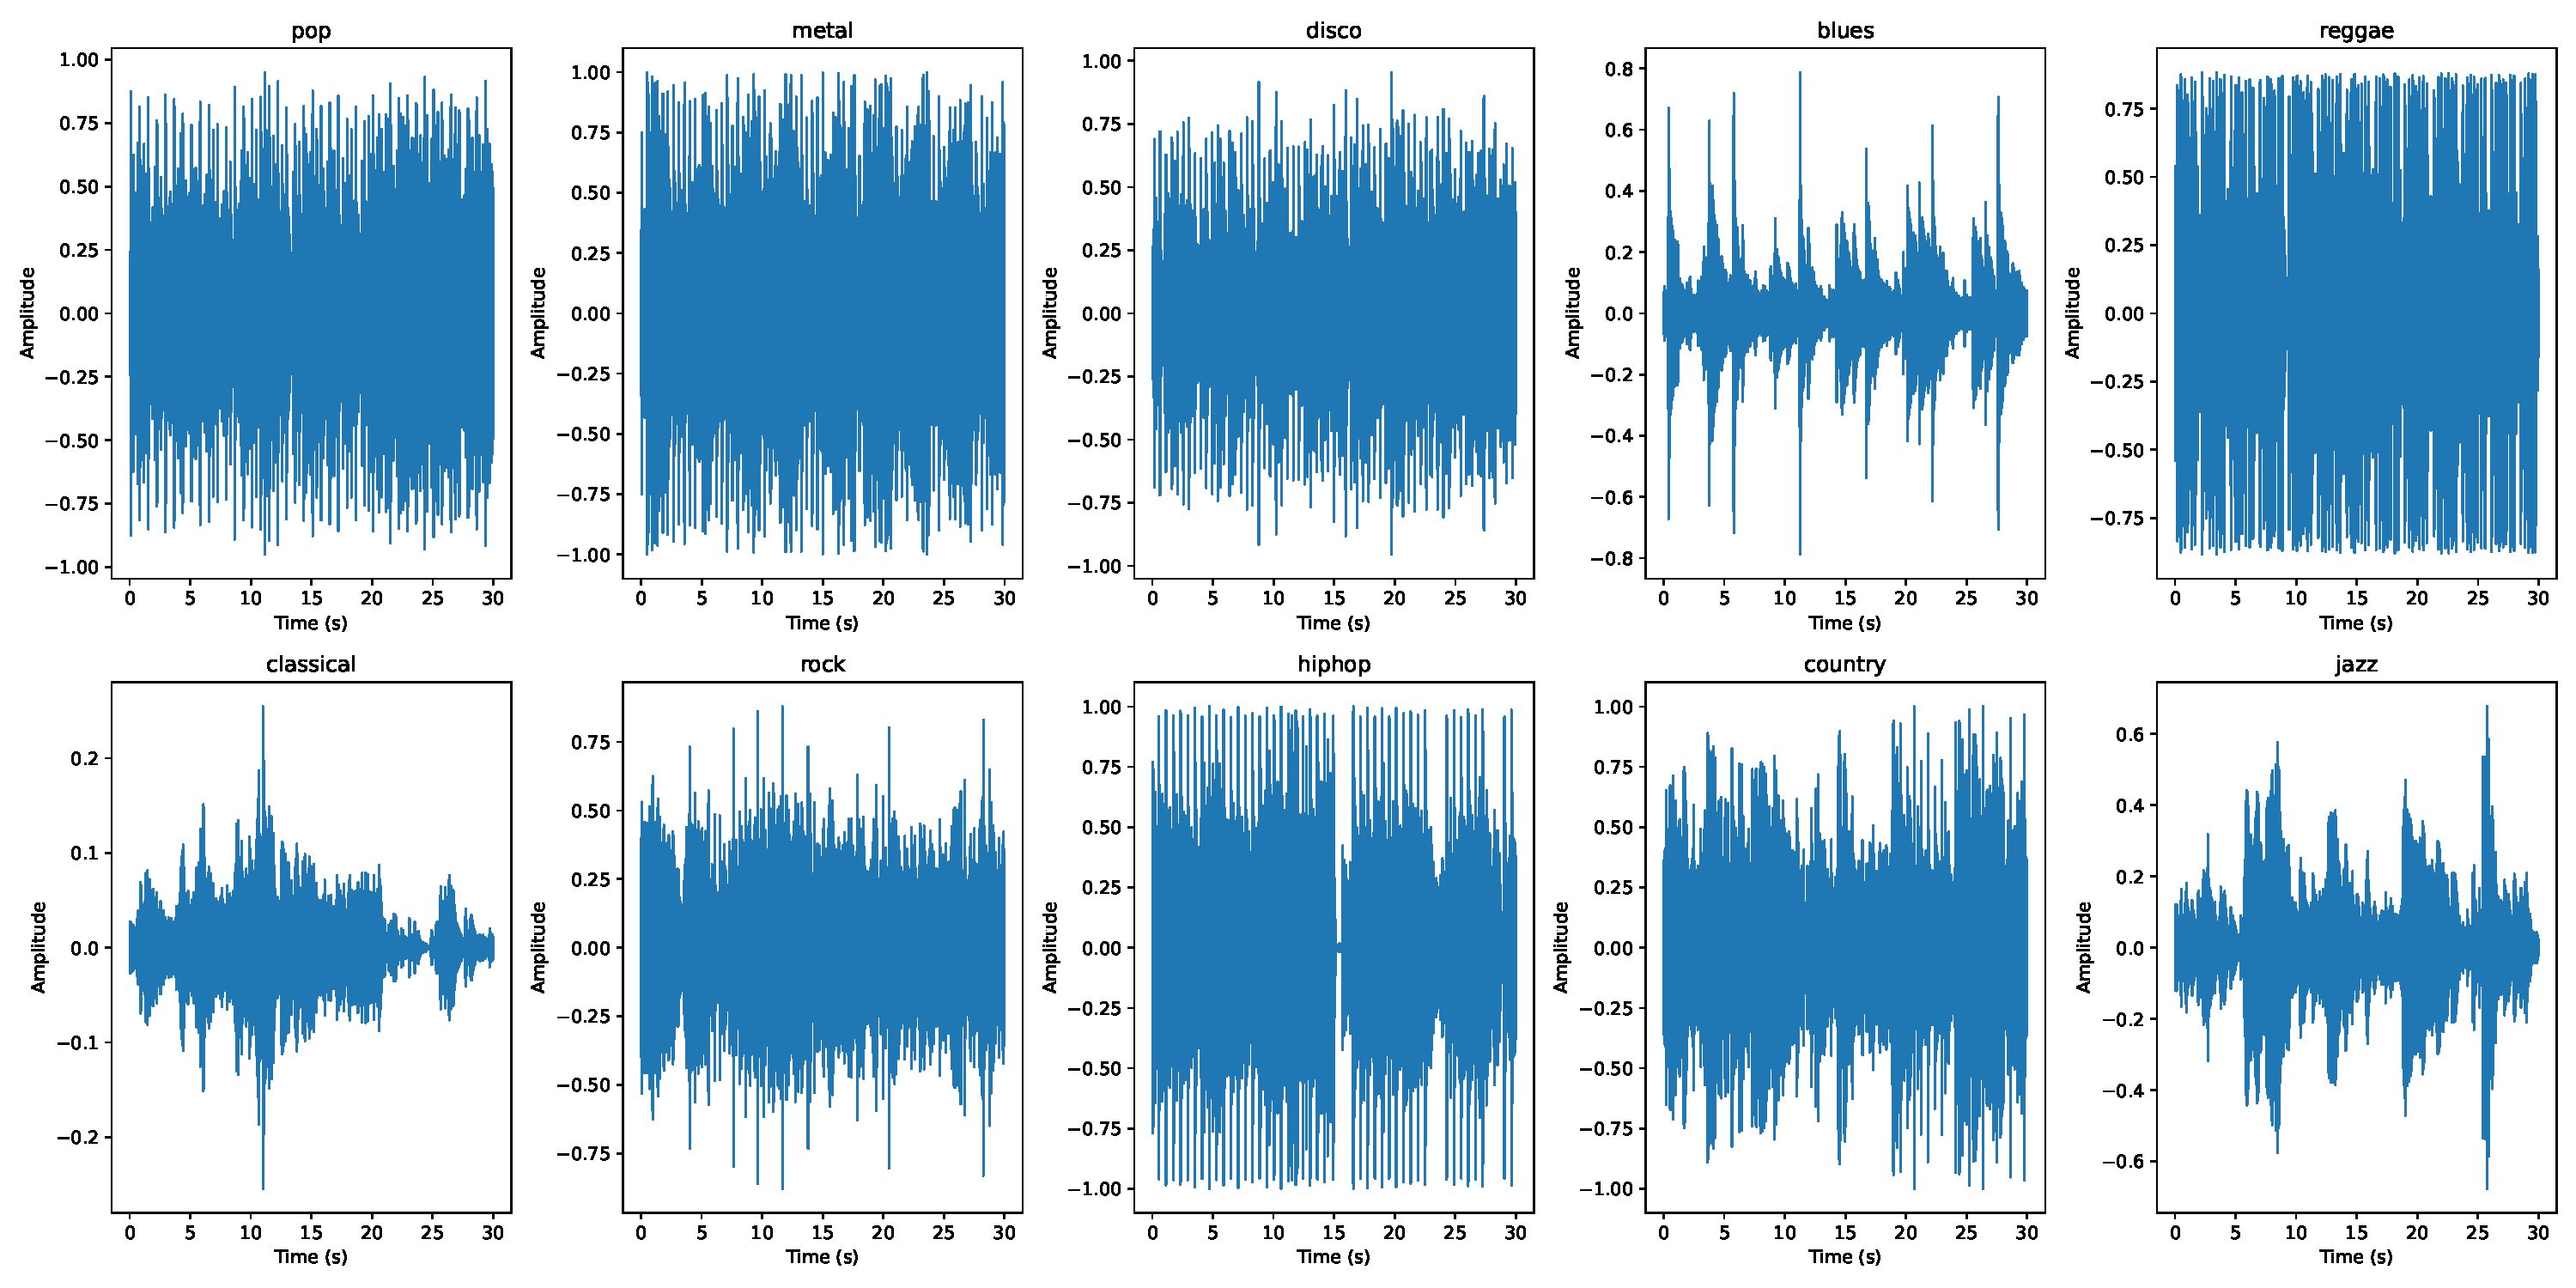
\includegraphics[width=0.9\textwidth]{graphics/waveform.pdf}
    \caption{Waveform of various sample audios track over time}
    \label{fig:waveform}
\end{figure}

\subsection{Chroma Analysis}
\textbf{Chroma features} (or chroma vectors) are audio features used in music information retrieval to represent the harmonic and tonal content of an audio signal. They capture the distribution of energy across the 12 different pitch classes (e.g., C, C\#, D, D\#, ..., B) regardless of octave. Figure \ref{fig:chroma} visualizes the changes in chroma features over time for a sample track. Each row corresponds to one pitch class, showing the energy present in that pitch class over time. Genres like rock, blues, pop, and hip-hop exhibit dense chroma activity, indicating frequent chord changes. In contrast, classical and jazz display more structured patterns, with jazz showing greater harmonic complexity.
\begin{figure}[h]
    \centering
    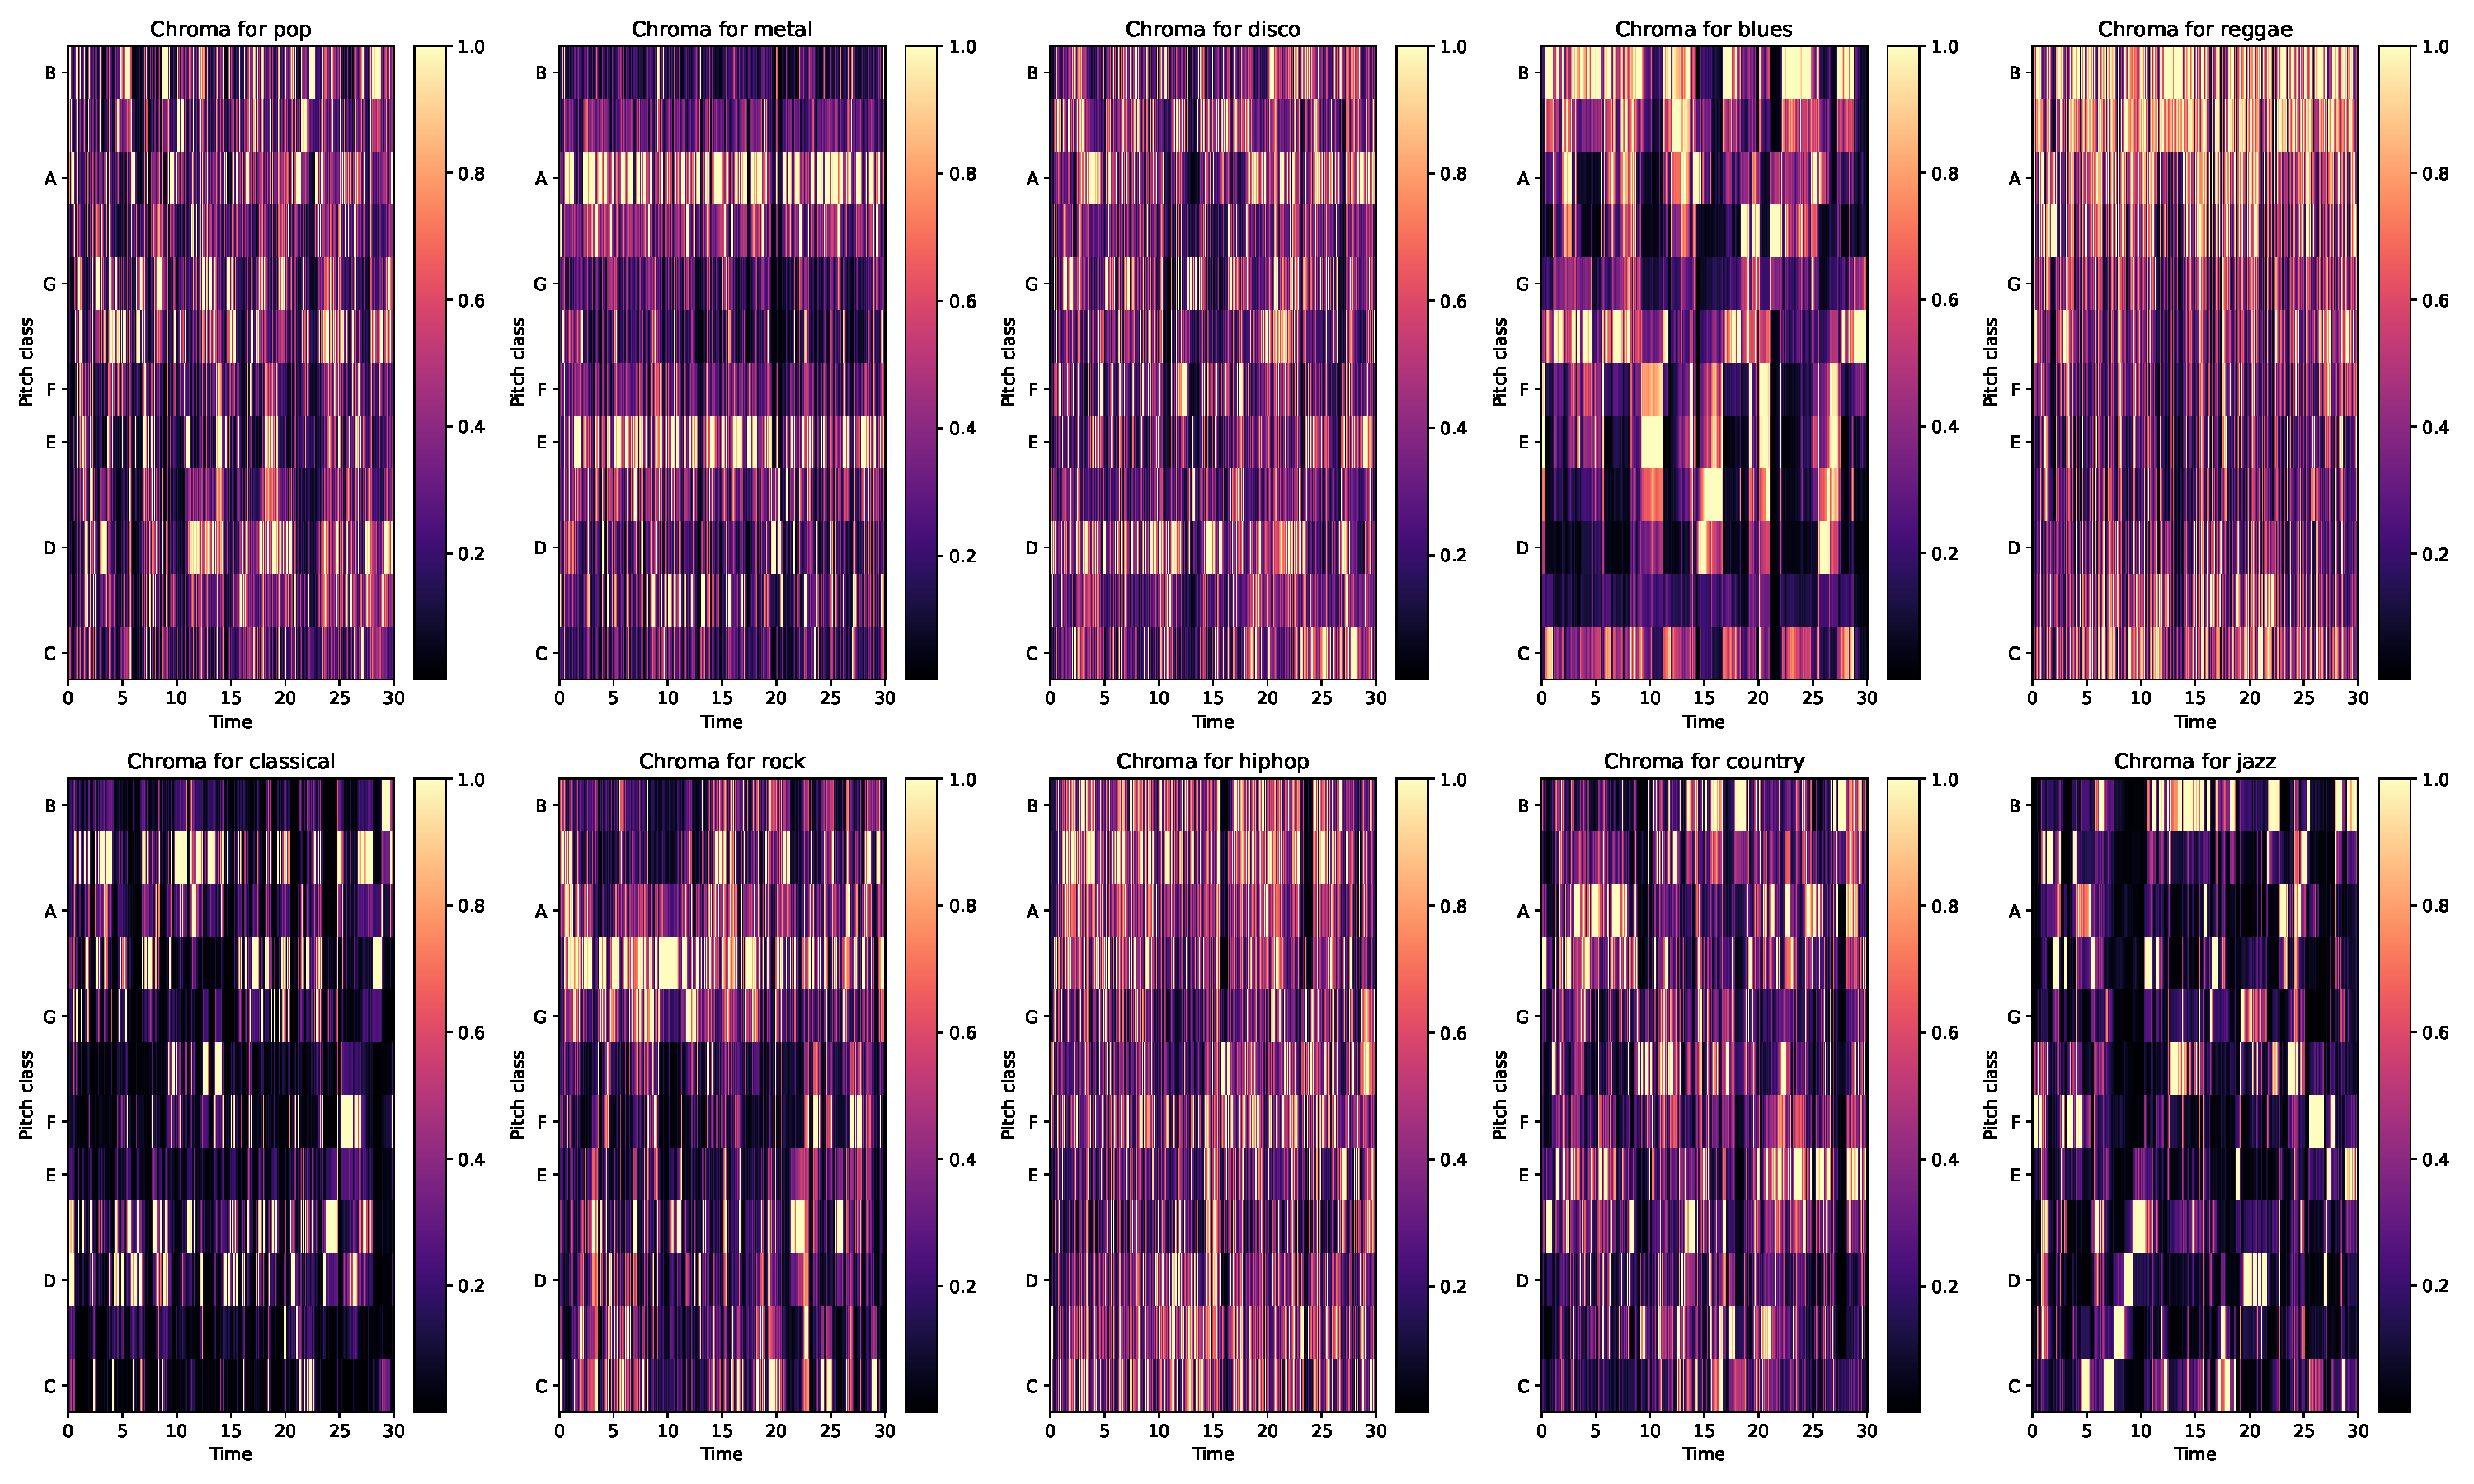
\includegraphics[width=0.9\textwidth]{graphics/chroma.pdf}
    \caption{Chroma Features of various pitch classes over time}
    \label{fig:chroma}
\end{figure}

\subsection{MFCC Analysis}
MFCCs (\text{Mel-Frequency Cepstral Coefficients}) are widely used in audio and speech processing for feature extraction. They convert raw audio signals into a compact, perceptually meaningful representation by simulating the human auditory system. Typically, the first 13-20 coefficients are used as features. Figure \ref{fig:mfcc} visualizes the MFCCs of a sample track. These coefficients capture the timbral properties of the audio signal, illustrating how the spectral content evolves over time. Genres such as rock, blues, and pop show high variability in MFCCs, reflecting their diverse timbral characteristics. In contrast, classical and jazz exhibit more structured patterns, indicating consistent timbral properties.
\begin{figure}[h]
    \centering
    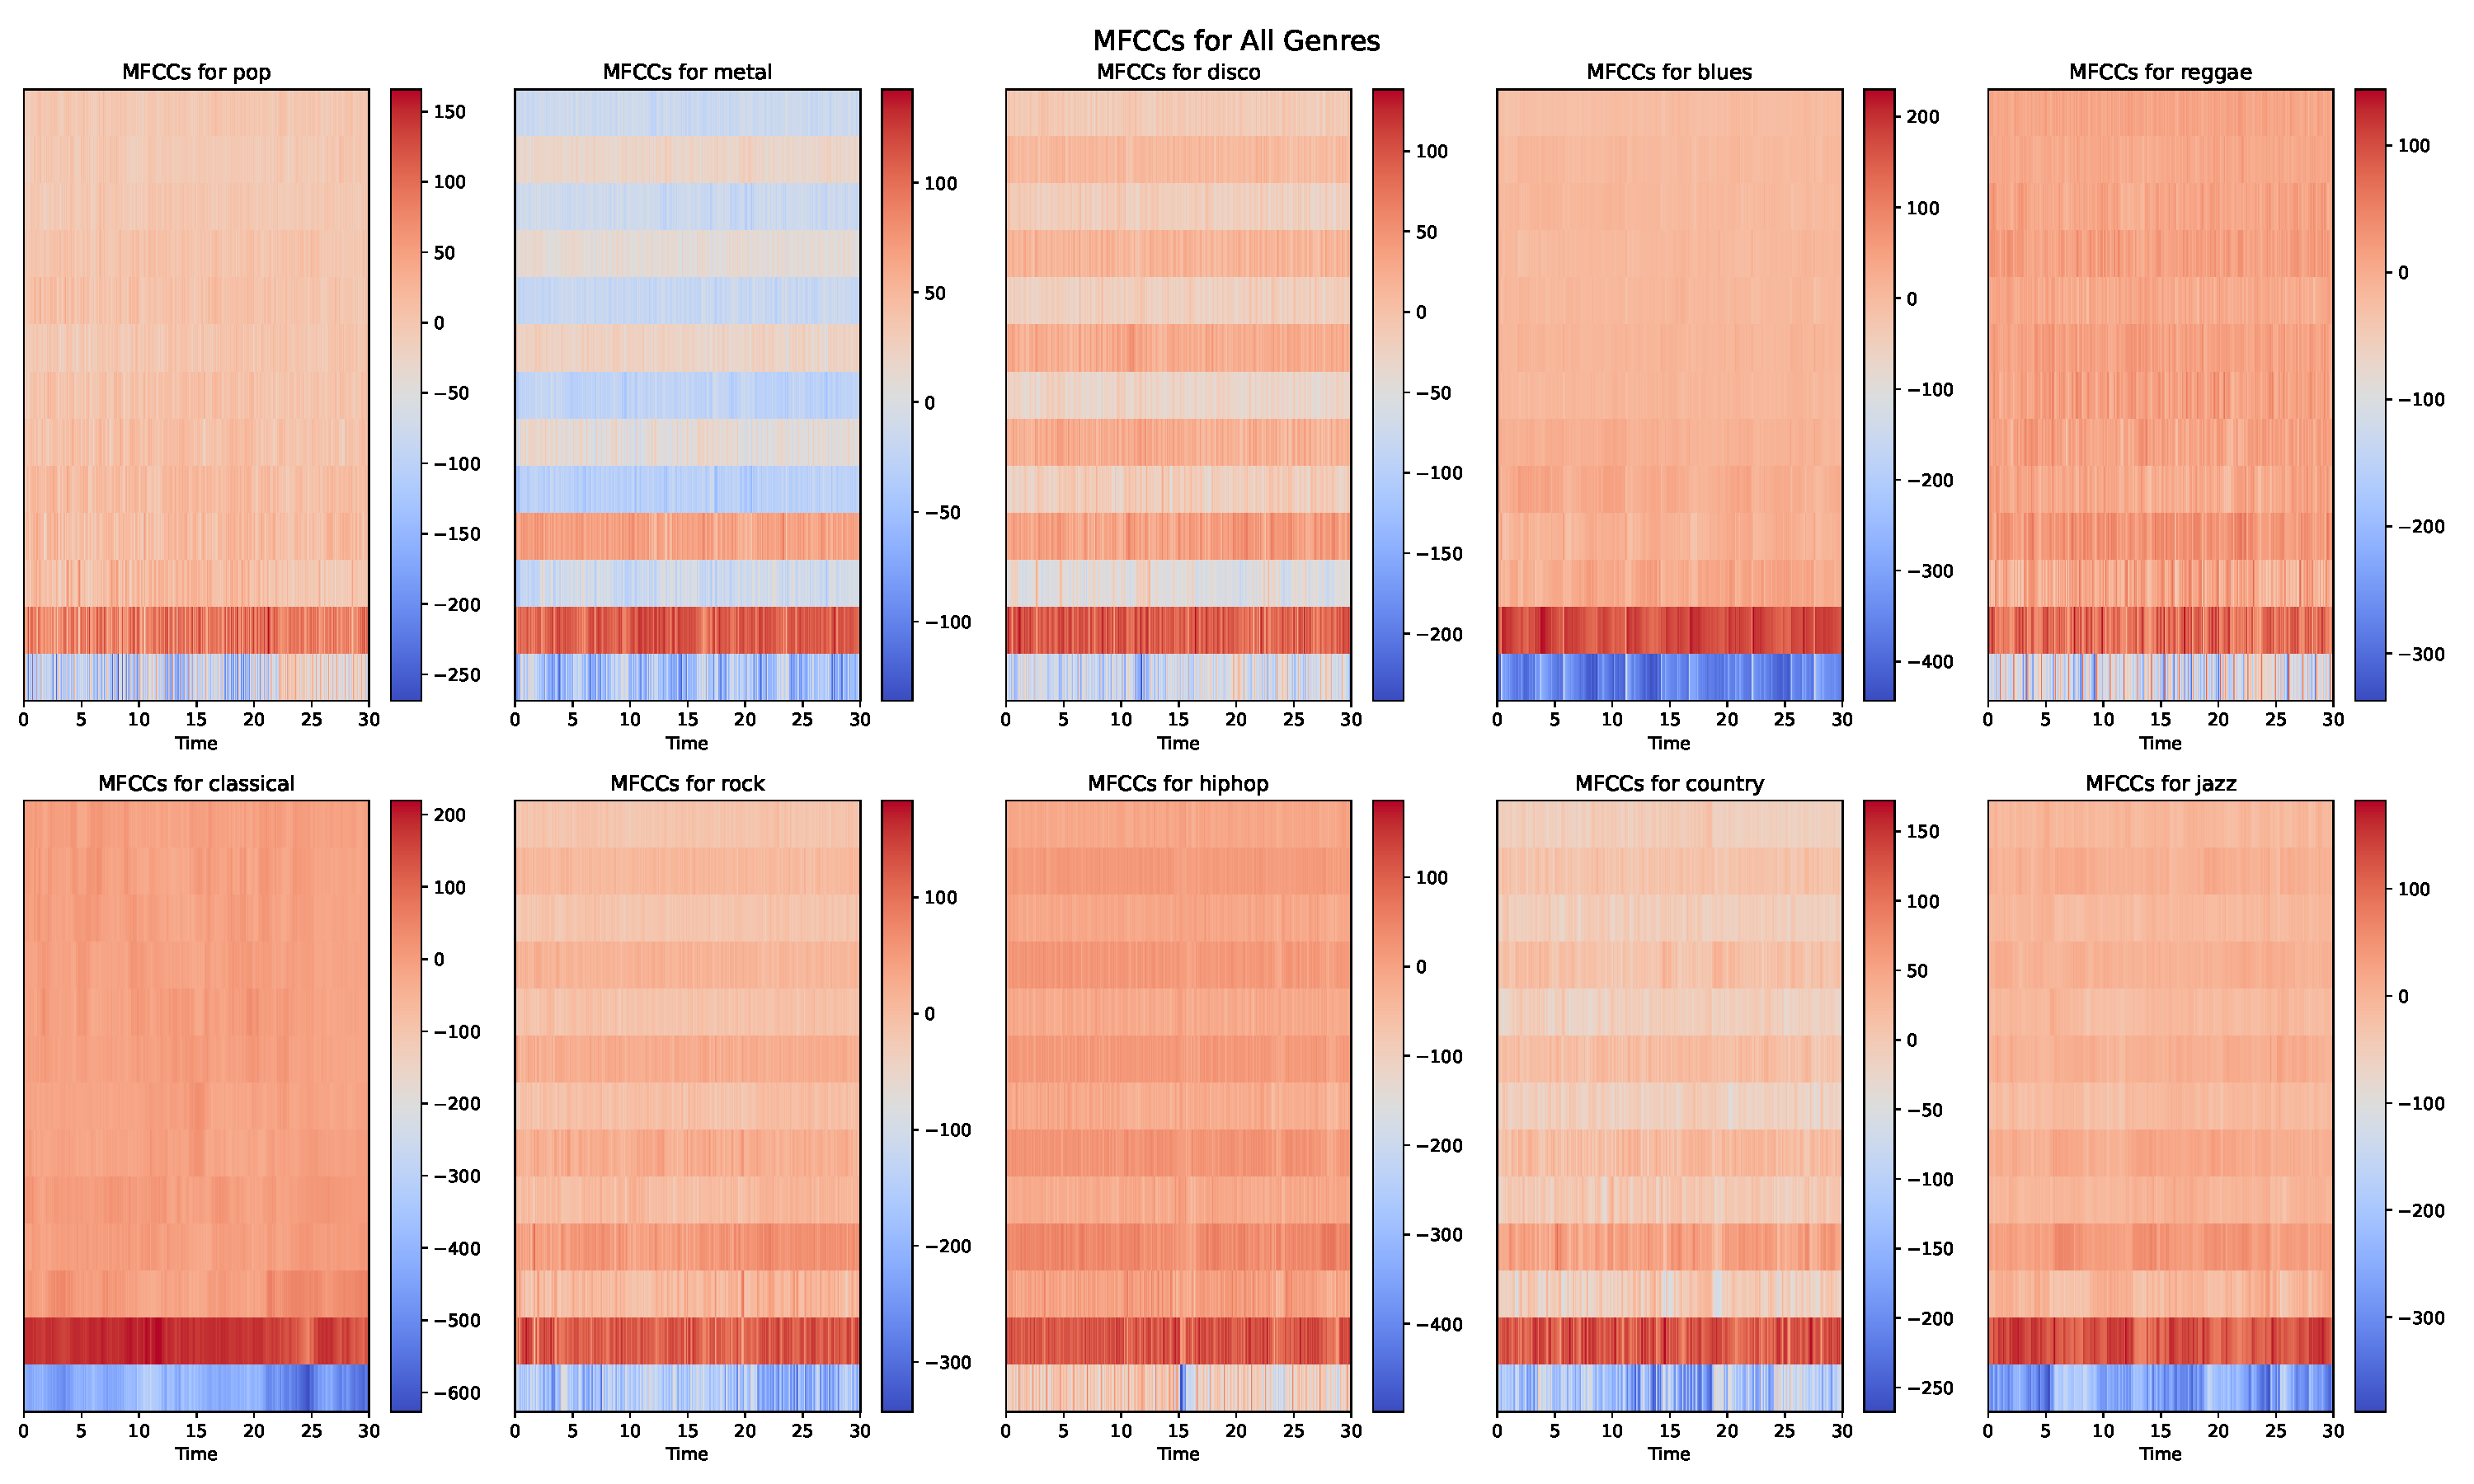
\includegraphics[width=0.9\textwidth]{graphics/mfccs.pdf}
    \caption{MFCC13 of various sample audios track over time}
    \label{fig:mfcc}
\end{figure}

\subsection{Mel Spectrogram Analysis}
A \textbf{Mel Spectrogram} is a visual representation of the frequency content of an audio signal over time, mapped to the Mel scale. It approximates the human ear's response to different frequencies, emphasizing lower frequencies (where humans are more sensitive) and compressing higher frequencies. Figure \ref{fig:spectrogram} visualizes the Mel spectrogram of sample tracks. The spectrogram captures the frequency content of the audio signal over time, showing how the energy is distributed across different frequency bands. Genres like rock, blues, and pop exhibit dense spectrogram activity, indicating a wide range of frequency components. In contrast, classical and jazz show more structured patterns, with jazz displaying greater frequency complexity.
\begin{figure}[h]
    \centering
    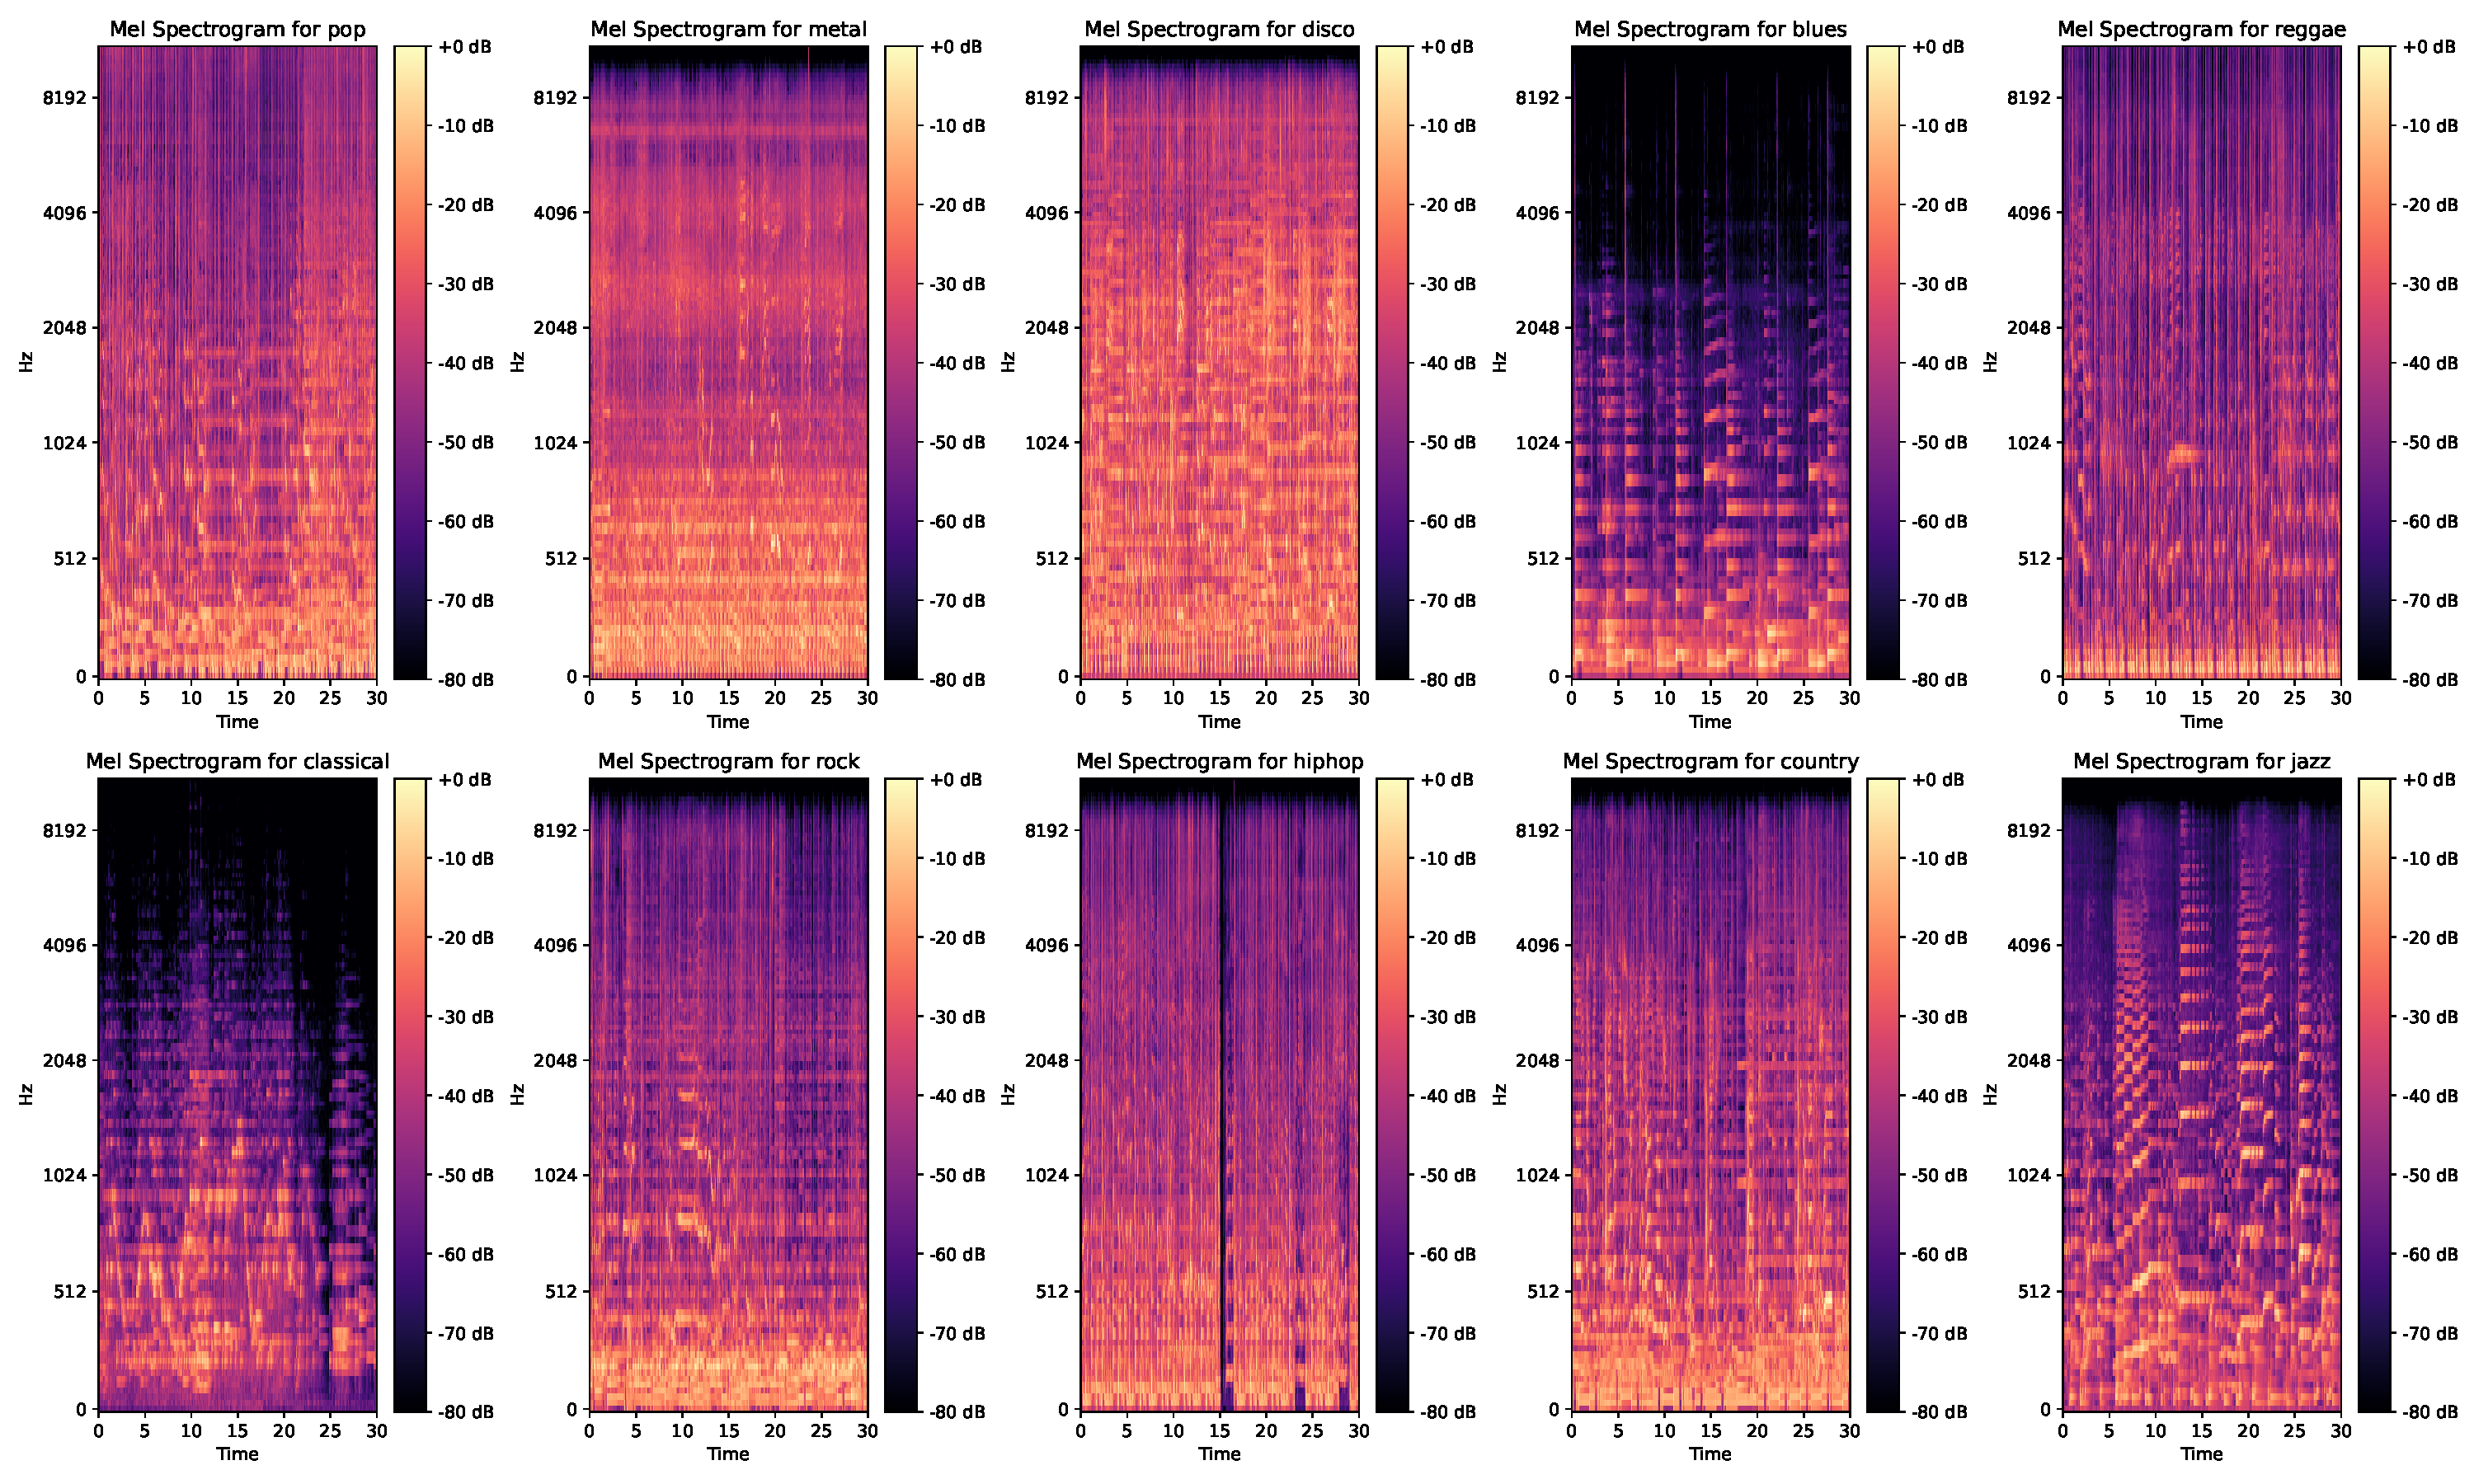
\includegraphics[width=0.9\textwidth]{graphics/mel.pdf}
    \caption{Mel Spectrogram of various sample audios track over time}
    \label{fig:spectrogram}
\end{figure}

\subsection{Principal Component Analysis}
Principal Component Analysis (PCA) is a dimensionality reduction technique that transforms data into a lower-dimensional space while preserving as much variance as possible. I applied PCA to the dataset and visualized the first two principal components in figure \ref{fig:pca}.
\begin{figure}[H]
    \centering
    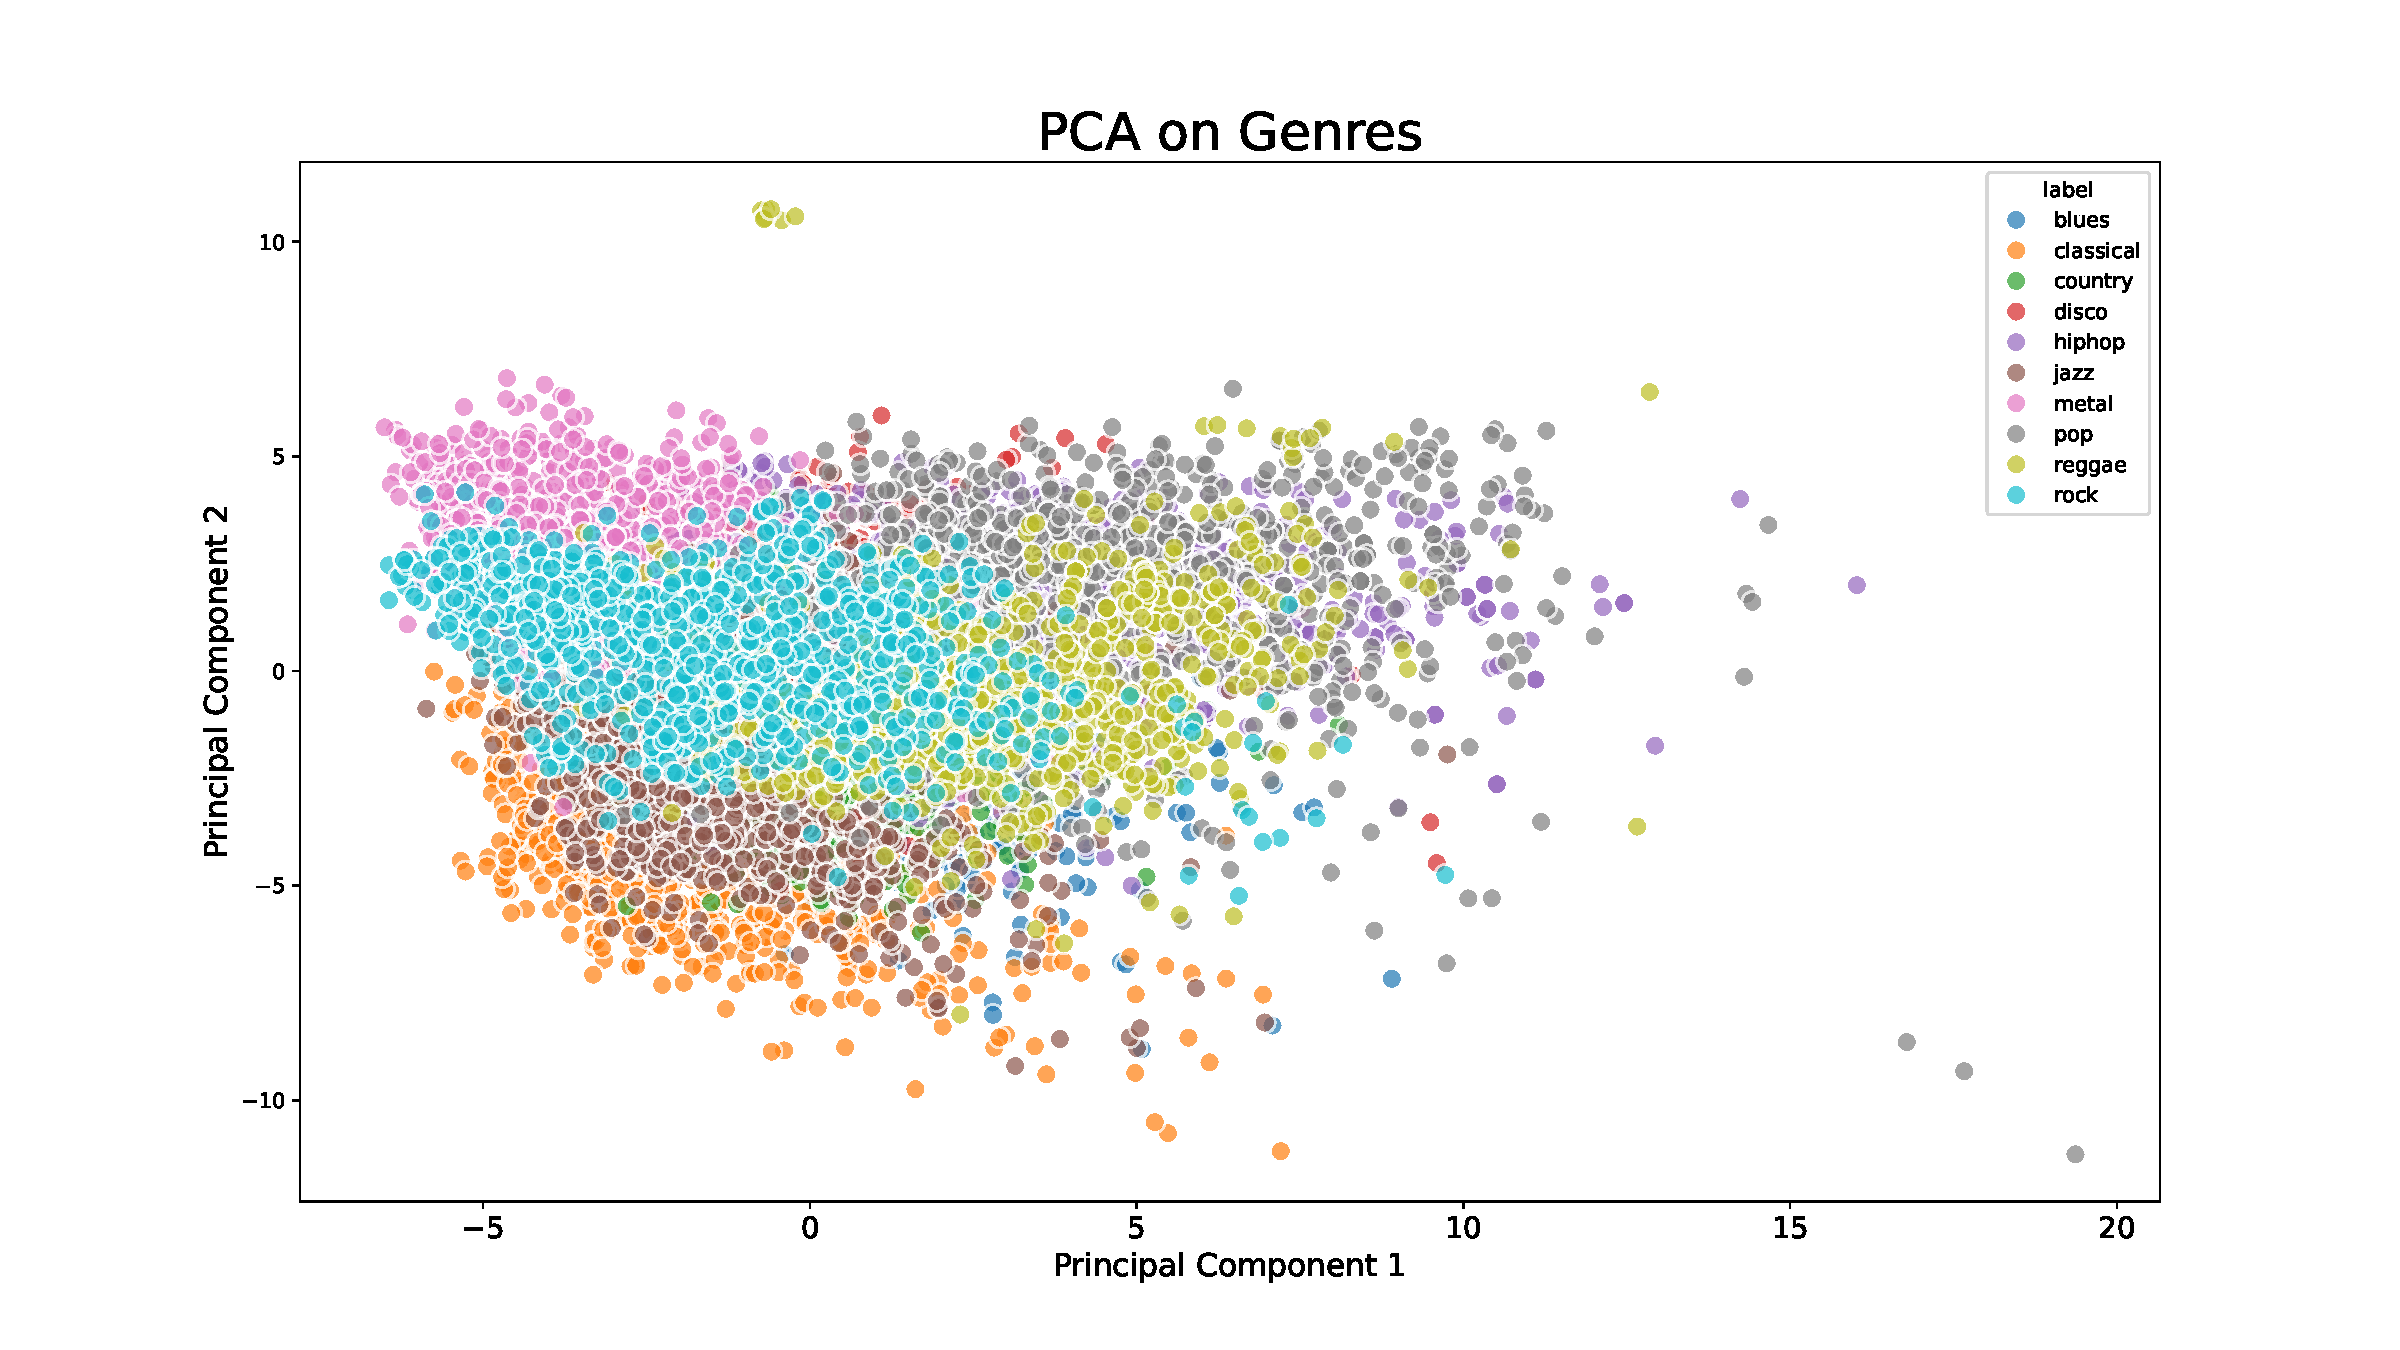
\includegraphics[width=0.9\textwidth]{graphics/pca.pdf}
    \caption{PCA of the GTZAN dataset}
    \label{fig:pca}
\end{figure}

\pagebreak

\section{Data Preprocessing} \label{sec:data_preprocessing}
\subsection{Normalization}
I normalized the features of the dataset to ensure that all features have the same scale. Normalization is essential for machine learning models that rely on distance-based metrics to prevent features with larger scales from dominating the model. I used min-max scaling to normalize the features. The formula for min-max scaling is:
\begin{equation}
    X_{\text{scaled}} = \frac{X - X_{\text{min}}}{X_{\text{max}} - X_{\text{min}}}
\end{equation}

\subsection{Train/Test Split} \label{sec:train_test_split}
I split the dataset into training and testing sets using an \textbf{8/2} split. I used the training set to train the model and the testing set to evaluate its performance. The validation has been used during the training phase of the classifers to find good values of the hyperparameters.

\subsection{Cross-Validation Split} \label{sec:cross_validation_split}
I used a 5-fold cross-validation split to evaluate the model's performance. Cross-validation is a technique used to assess the model's generalization performance by training and testing the model on different subsets of the data, as shown in figure \ref{fig:cross_validation}.
\begin{figure}[H]
    \centering
    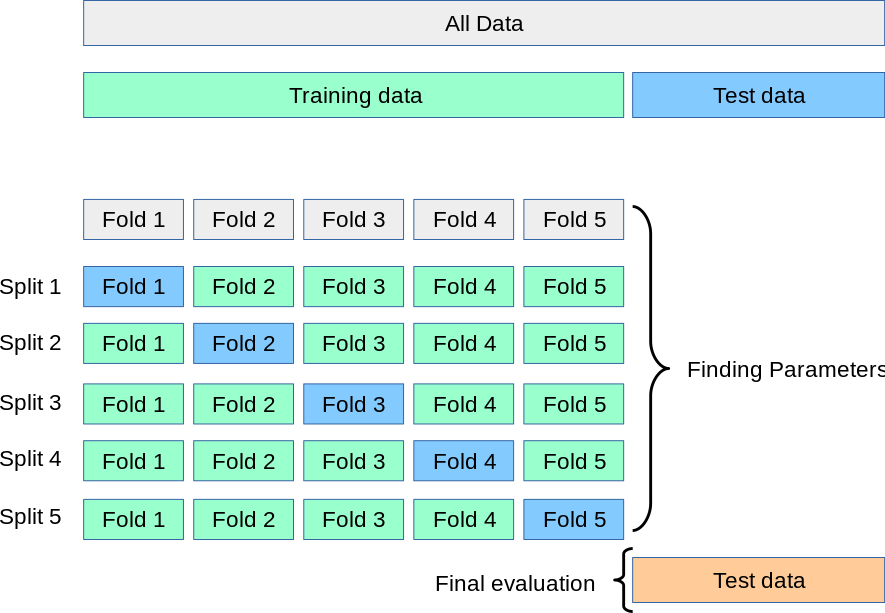
\includegraphics[width=0.5\textwidth]{graphics/grid_search_cross_validation.png}
    \caption{5-fold Cross-Validation Split\cite{31CrossvalidationEvaluating}}
    \label{fig:cross_validation}
\end{figure}

\subsection{One-Hot Encoding}
For CNN model, I used \textbf{one-hot encoding} to convert the target labels into a binary matrix. One-hot encoding is a technique used to convert categorical data into a binary matrix, where each column represents a unique category, and each row represents an instance. For example, the label 'rock' would be encoded as [0, 0, 0, 1, 0, 0, 0, 0, 0, 0] in a 10-class classification problem.

\pagebreak
\section{Traditional Machine Learning Models} \label{sec:traditional_ml}
\subsection{Baseline Models}
I trained several traditional machine learning models on the dataset to establish a baseline performance. The models I used are:
\begin{itemize}
    \item \textbf{Logistic Regression}
    \item \textbf{Support Vector Machine}
    \item \textbf{Decision Tree}
    \item \textbf{Random Forest}
    \item \textbf{XGBoost}
\end{itemize}
The models were trained using the default hyperparameters and evaluated using 5-fold cross-validation. The results on the training set are summarized in figure \ref{fig:baseline_models}, with the x-axis representing accuracy. The \textbf{XGBoost} model outperformed the other models, achieving an accuracy of \textbf{0.91} on the training set.
\begin{figure}[H]
    \centering
    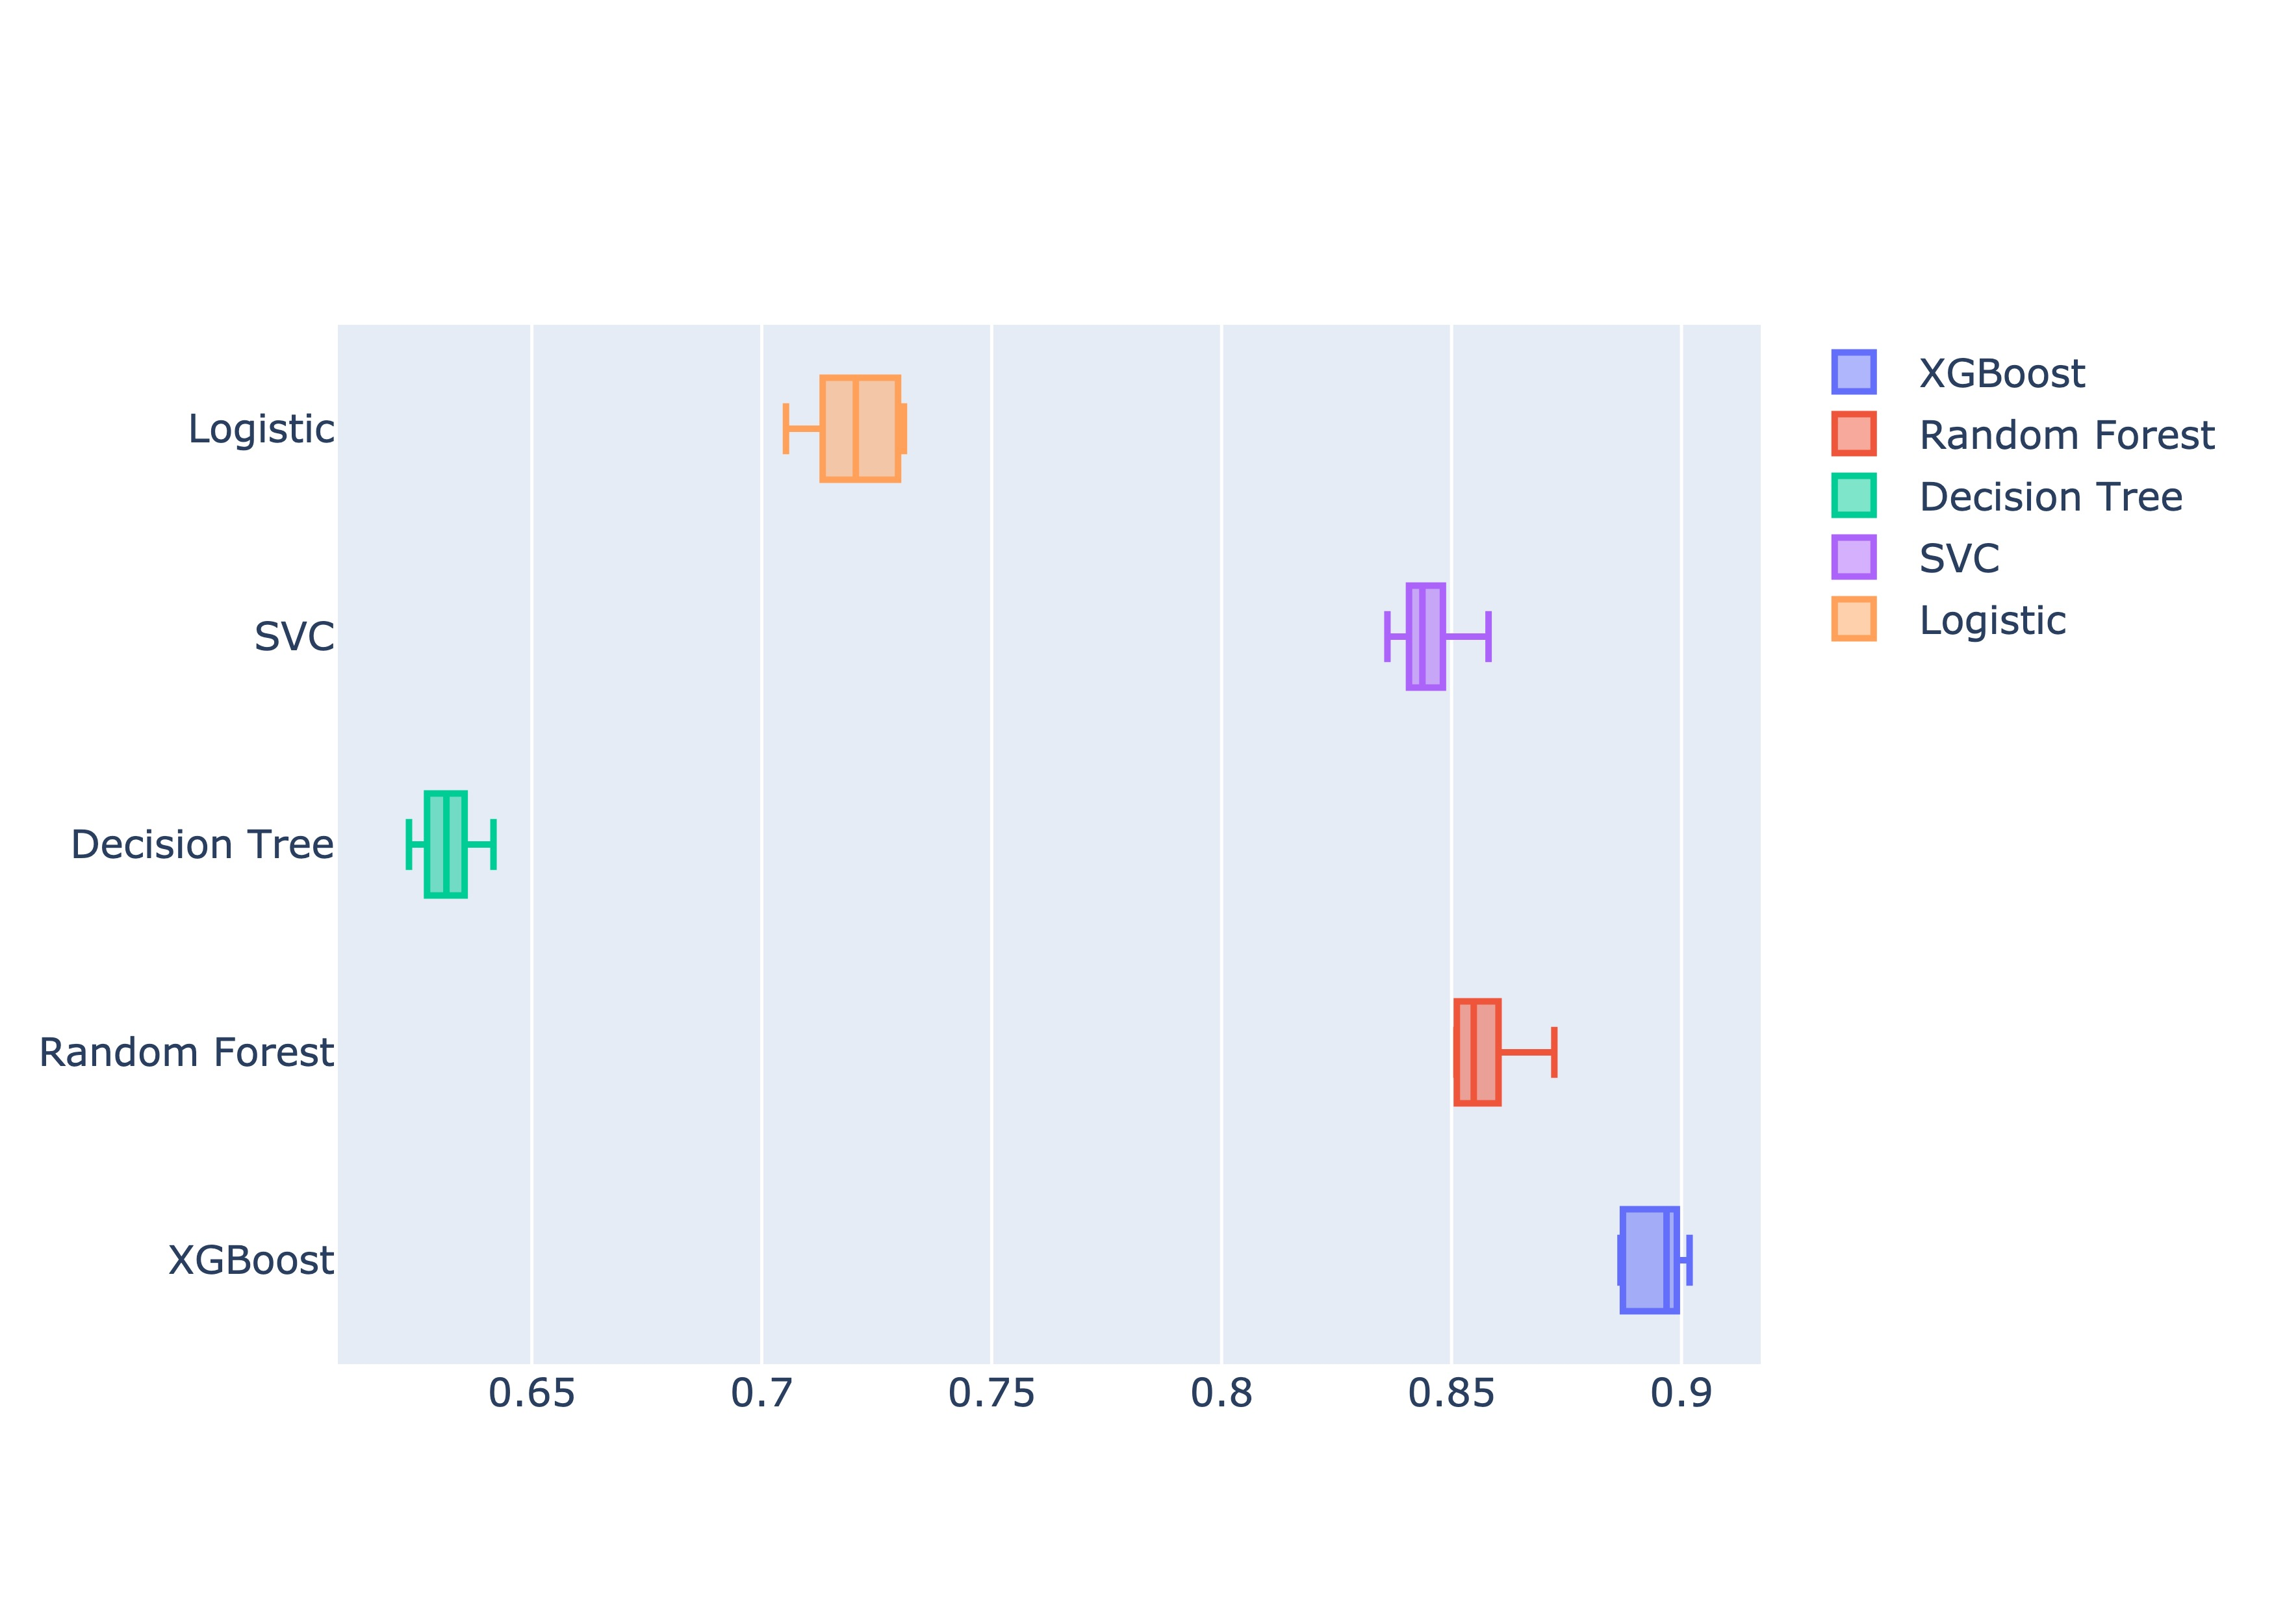
\includegraphics[width=0.9\textwidth]{graphics/baseline_models.jpg}
    \caption{Baseline Models Performance on training set}
    \label{fig:baseline_models}
\end{figure}

\subsection{Model Evaluation}
I evaluated the XGBoost model on the testing set and obtained an accuracy of \textbf{0.90}. The confusion matrix in figure \ref{fig:xgboost_evaluation} shows that the model performs well for some genres (e.g., classical, metal) but struggles with others (e.g., rock, country).
\begin{figure}[H]
    \centering
    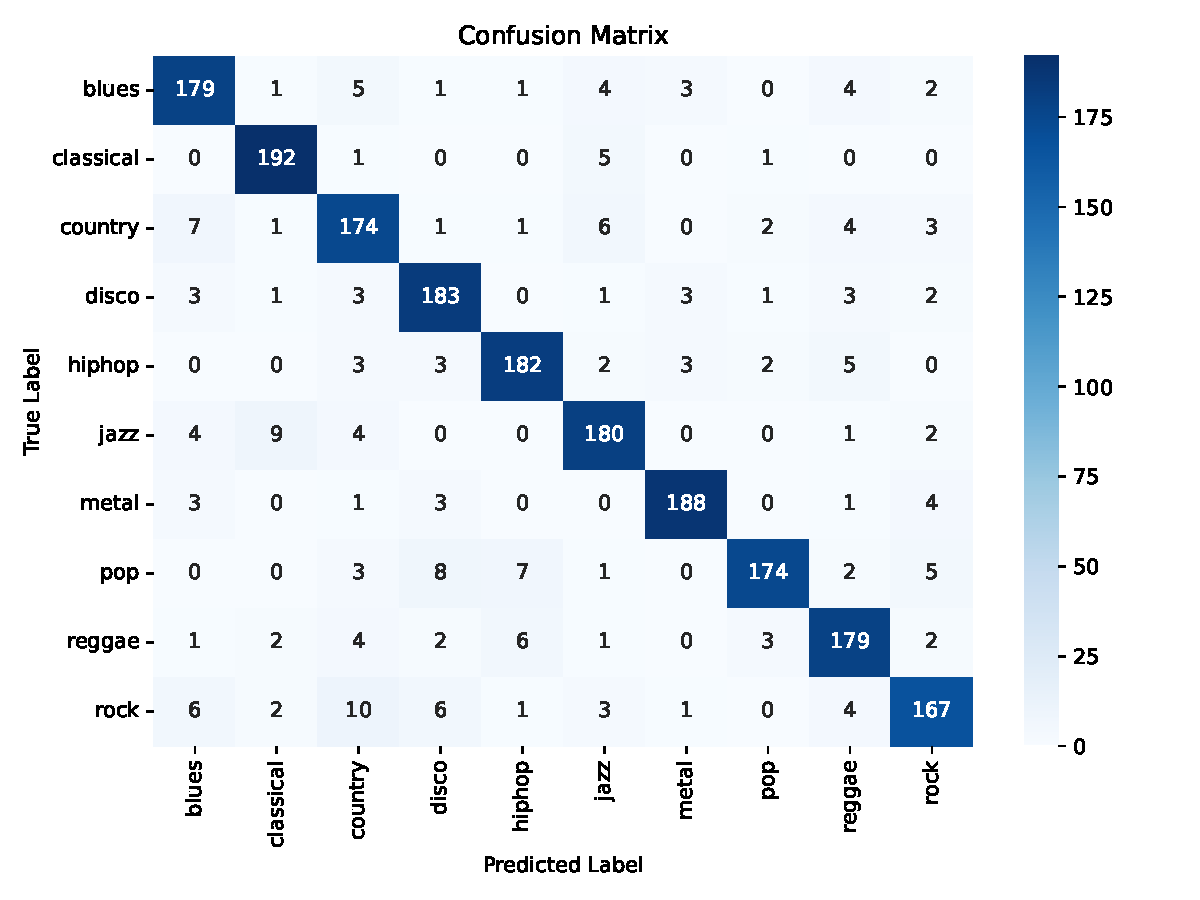
\includegraphics[width=0.9\textwidth]{graphics/confusion_matrix.pdf}
    \caption{XGBoost Model Evaluation on testing set}
    \label{fig:xgboost_evaluation}
\end{figure}

\subsection{Hyperparameter Tuning}
I used \textbf{RandomizedSearchCV} to tune the hyperparameters of the XGBoost model. I performed a randomized search over a predefined hyperparameter grid and selected the best hyperparameters based on the model's performance. The hyperparameters I tuned were:
\begin{itemize}
    \item \textbf{max\_depth}: Maximum depth of the tree
    \item \textbf{learning\_rate}: Step size shrinkage used in update to prevent overfitting
    \item \textbf{n\_estimators}: Number of boosting rounds
    \item \textbf{subsample}: Subsample ratio of the training instances
    \item \textbf{reg\_alpha}: L1 regularization term on weights
\end{itemize}
The best hyperparameters found by RandomizedSearchCV were:
\begin{itemize}
    \item \textbf{max\_depth}: 5
    \item \textbf{learning\_rate}: 0.2
    \item \textbf{n\_estimators}: 500
    \item \textbf{subsample}: 0.8
    \item \textbf{reg\_alpha}: 0.1
\end{itemize}

\pagebreak
\section{Convolutional Neural Network (CNN)} \label{sec:cnn}
Deep learning enables music genre classification without relying on manually crafted features. In this study, audio signals are transformed into spectrograms, which are then treated as images for classification.

\subsection{Spectrogram Generation}
A \textbf{spectrogram} is a 2D representation of a signal, having time on the x-axis, \textbf{frequency} on the y-axis. Each audio signal was converted into a MEL spectrogram. The parameters used to generate the power spectrogram using STFT are listed below:
\begin{itemize}
    \item \textbf{Window size}: 2048 samples
    \item \textbf{Hop length}: 512 samples
    \item \textbf{Sampling rate}: 22050 Hz
\end{itemize}

\subsection{Cost Function}
The cost function used in this study is the categorical cross-entropy loss function, which is commonly used in multi-class classification problems. The categorical cross-entropy loss function is defined as:
\begin{equation}
    L(y, \hat{y}) = -\sum_{i} y_i \log(\hat{y}_i)
\end{equation}
where $y$ is the true label, $\hat{y}$ is the predicted label, and $i$ is the class index.

\subsection{Metrics}
The model's performance was evaluated using the following metrics:
\begin{itemize}
    \item \textbf{Accuracy}: The ratio of correctly classified instances to the total instances
    \item \textbf{Precision}: The ratio of true positive instances to the total predicted positive instances
    \item \textbf{Recall}: The ratio of true positive instances to the total actual positive instances
    \item \textbf{F1-score}: The harmonic mean of precision and recall
\end{itemize}

\subsection{Model Architecture}
\textbf{Mel spectrograms} can be treated as images and used as input to a CNN, which excels in image classification tasks. Each block in the CNN consists of the following layers:
\begin{itemize}
    \item \textbf{Convolutional 2D layer}: Extracts features from the input image using filters. Each filter slides over the image and performs a convolution operation, producing a feature map that highlights different aspects of the image, such as edges, textures, or patterns.
    \item \textbf{Max pooling layer}: Reduces the spatial dimensions of the feature map by sliding a window over the feature map and taking the maximum value within the window. This operation helps in reducing the computational load and makes the features more robust to spatial variations.
    \item \textbf{Dropout layer}: Regularizes the model to prevent overfitting by randomly setting a fraction of the input units to zero at each update during training. This encourages the model to learn more robust features.
\end{itemize}

The architecture of the CNN model \cite{ghildiyalMusicGenreClassification2020} used in this study is shown in figure \ref{fig:cnn_architecture}.
\begin{figure}[H]
    \centering
    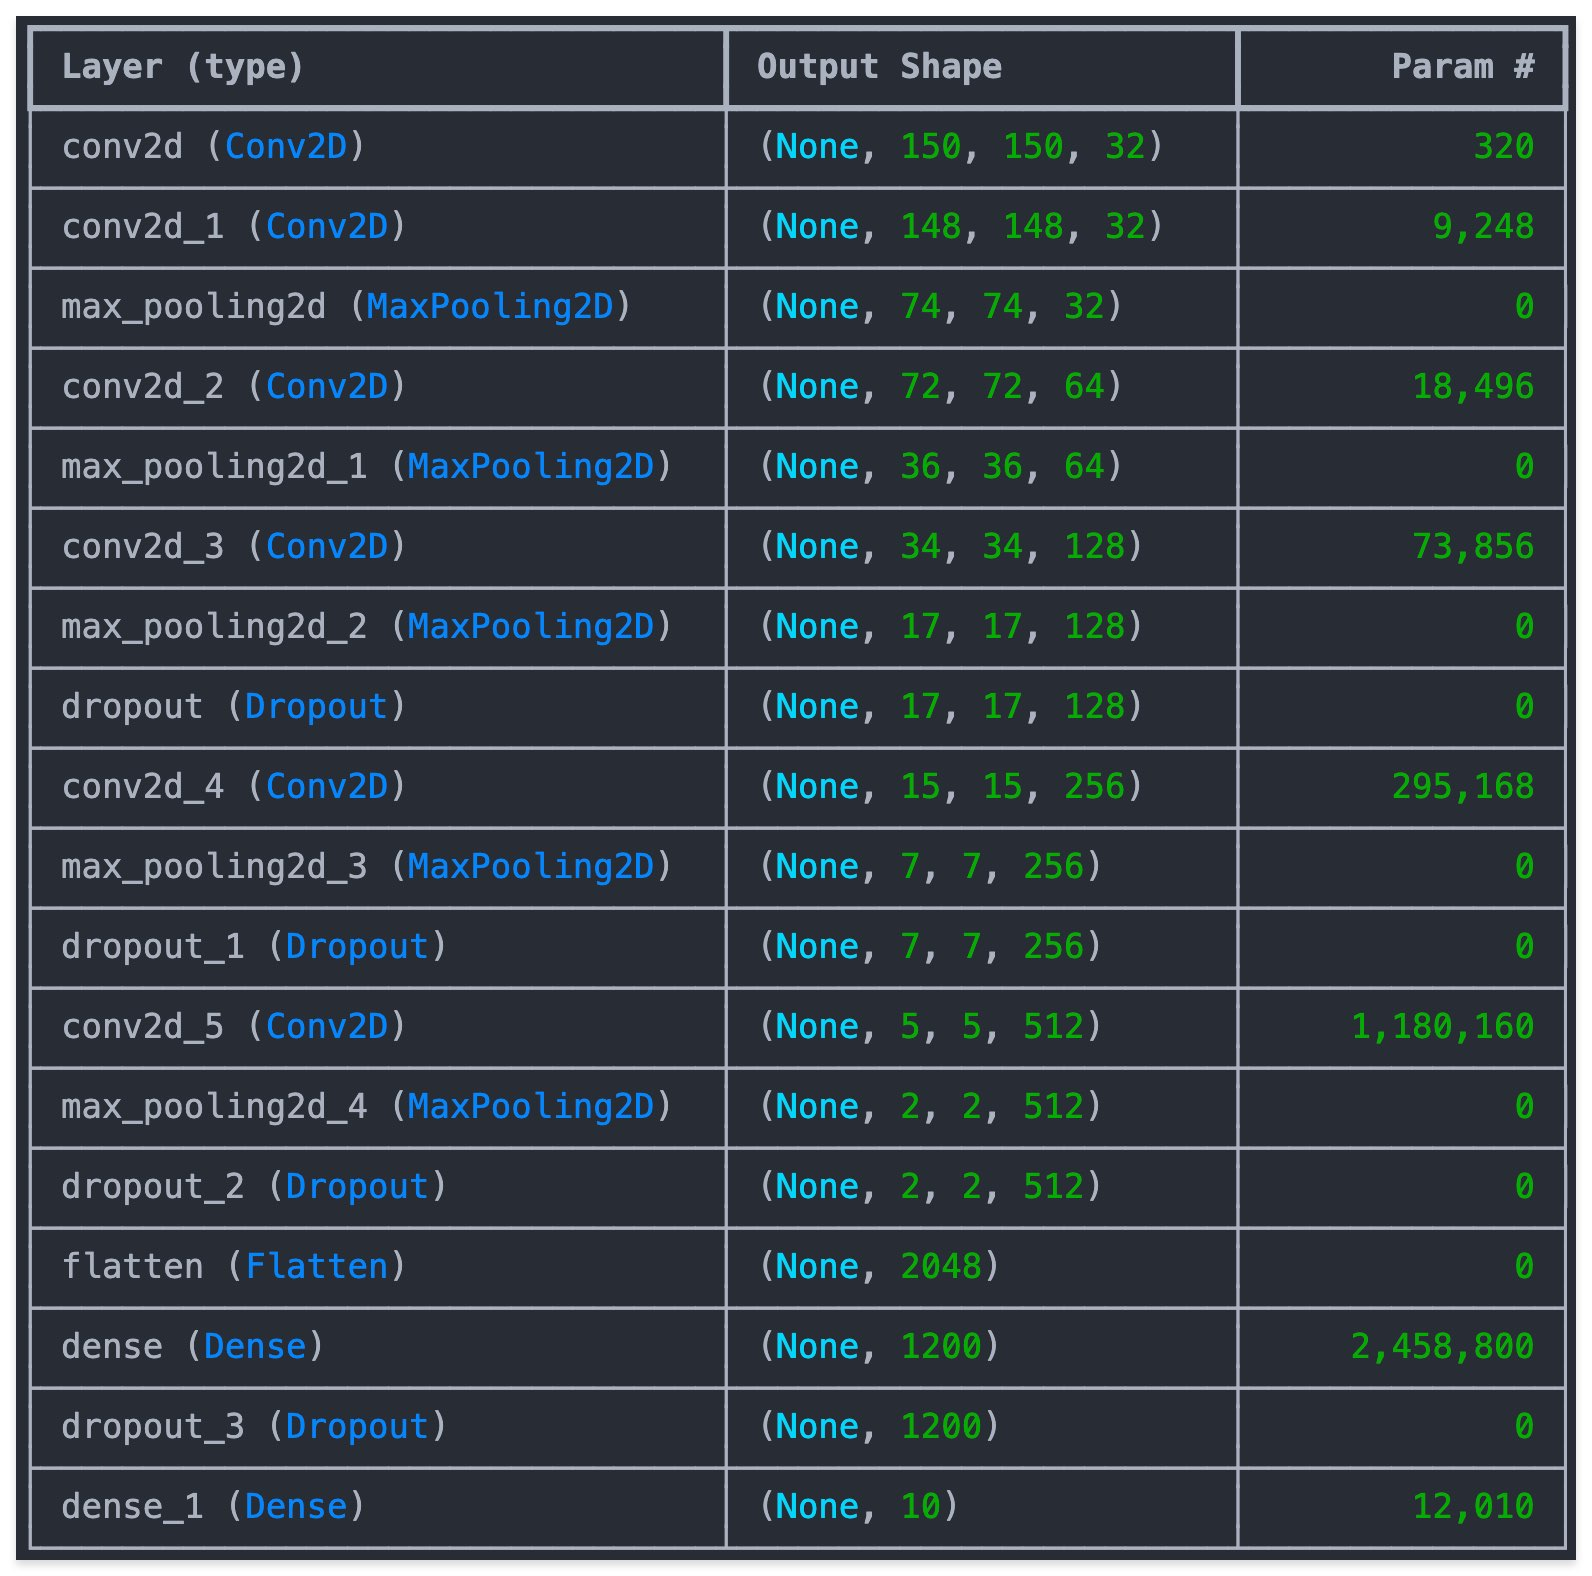
\includegraphics[width=0.9\textwidth]{graphics/model_architecture.jpg}
    \caption{CNN Model Architecture}
    \label{fig:cnn_architecture}
\end{figure}

\subsection{Model Training}
The CNN model was trained using the training set and validated using the validation set. The model was trained for 50 epochs with a batch size of 32. The model was compiled using the \textbf{Adam optimizer}(with learning rate $=0.0001$) and the categorical cross-entropy loss function.

The training phase results are depicted in figure \ref{fig:loss_accuracy}, showing the loss and accuracy curves. The figure illustrates a decreasing loss and increasing accuracy over time, indicating effective learning. However, as the number of epochs increases, there is a risk of \textbf{overfitting}.
\begin{figure}[H]
    \centering
    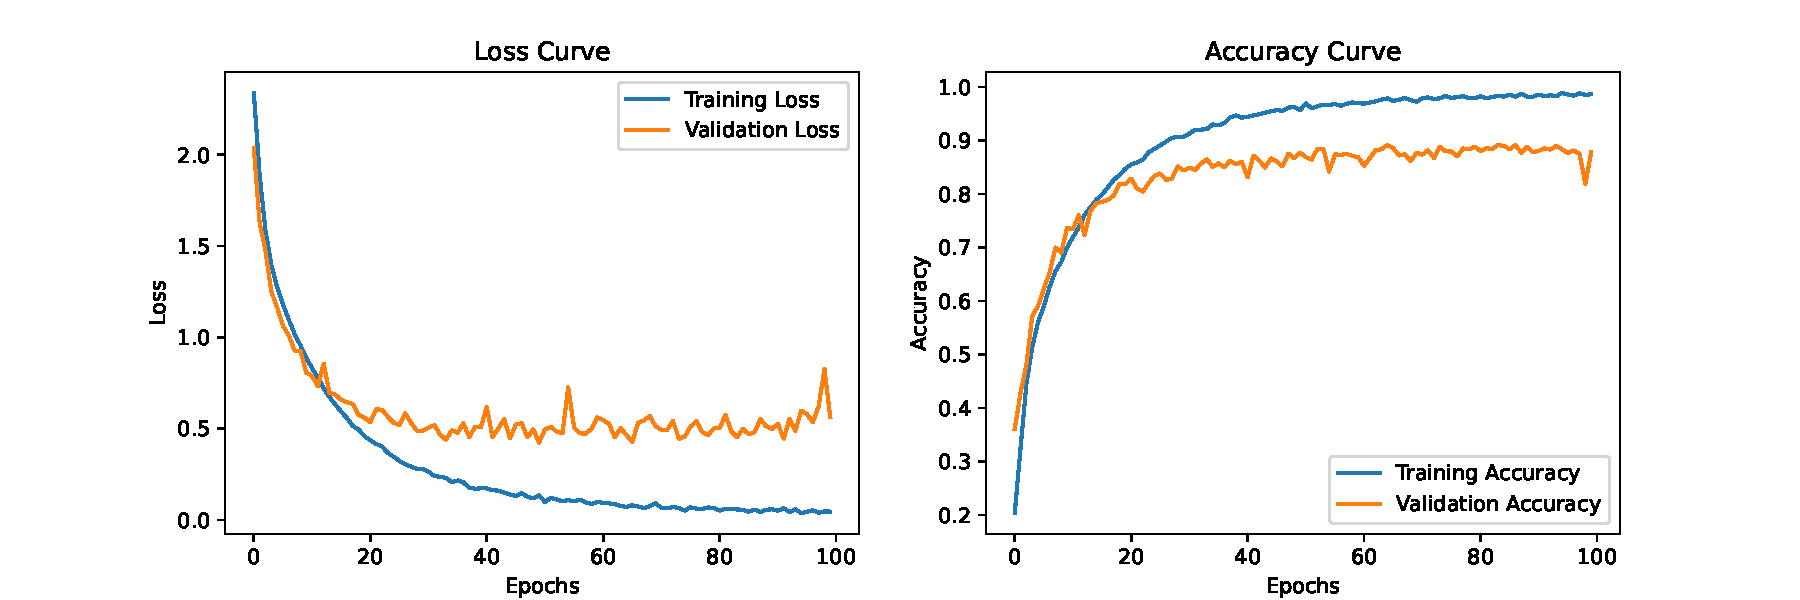
\includegraphics[width=0.9\textwidth]{graphics/loss_accuracy.pdf}
    \caption{Loss and Accuracy Curves during training}
    \label{fig:loss_accuracy}
\end{figure}

\subsection{Model Evaluation}
The CNN model was trained on the training set and evaluated on the testing set. It achieved an accuracy of \textbf{0.87} on the testing set. The confusion matrix in figure \ref{fig:cnn_evaluation} indicates that the CNN model performs well for most genres. However, it encounters difficulties with genres like jazz and reggae, which exhibit similar spectral characteristics.
\begin{figure}[H]
    \centering
    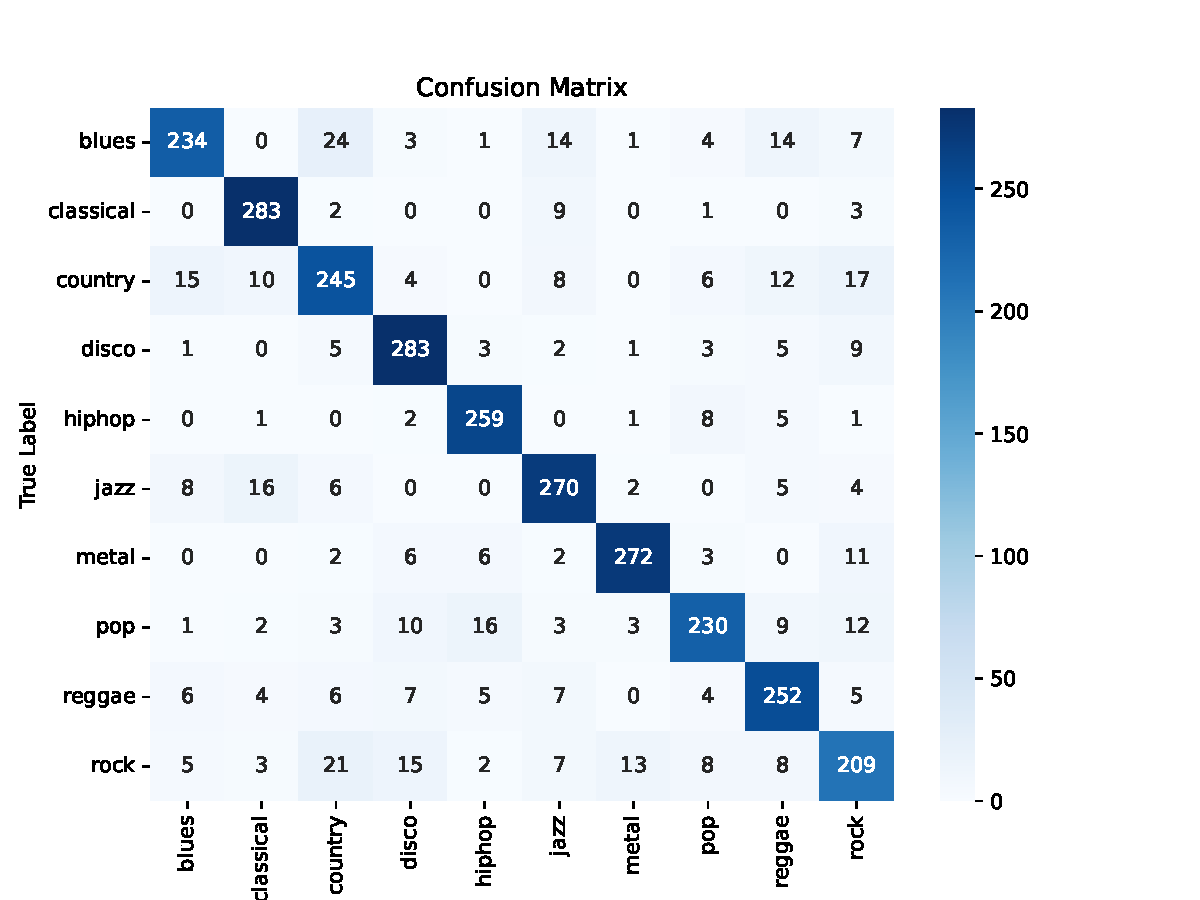
\includegraphics[width=0.9\textwidth]{graphics/cnn_evaluation.pdf}
    \caption{CNN Model Evaluation on testing set}
    \label{fig:cnn_evaluation}
\end{figure}

\section{Conclusion} \label{sec:conclusion}
In this study, I explored the GTZAN dataset, preprocessed the data, and trained both traditional machine learning models and a CNN model for music genre classification. The CNN model underperformed compared to traditional models because CNNs are optimized for spatial data, and when applied to extracted audio features that lack spatial relationships, they struggle. On the other hand, traditional models like SVC and XGBoost utilize manually extracted features (such as MFCC, Chroma, Spectral Contrast, Zero-Crossing Rate, etc.) that are specifically designed to capture audio patterns effectively. SVC and XGBoost classify based on these high-dimensional features efficiently and are less prone to overfitting.

Based on the performance table \ref{tab:performance}, it is evident that \textbf{XGBoost} is the most suitable model for this classification task.
\begin{table}[h]
    \centering
    \begin{tabular}{ccccc}
        \toprule
        \textbf{Model} & \textbf{Accuracy} & \textbf{Precision} & \textbf{Recall} & \textbf{F1\-score} \\
        \midrule
        SVC            & 0.85              & 0.85               & 0.85            & 0.85               \\
        Random Forest  & 0.87              & 0.87               & 0.87            & 0.87               \\
        CNN            & 0.87              & 0.87               & 0.87            & 0.87               \\
        XGBoost        & 0.91              & 0.91               & 0.91            & 0.91               \\
        \bottomrule
    \end{tabular}
    \caption{Model Performance on testing set}
    \label{tab:performance}
\end{table}

\clearpage
\printbibliography[heading=bibintoc, title = {References}]
\end{document}